\documentclass{article}
\usepackage{tikz, comment}
\usepackage{pifont}
\usepackage{fontspec}
\usetikzlibrary{arrows, decorations.markings, decorations.pathreplacing}
\begin{comment}
:Title: Not defined yet
:Slug: No name yet

Description Here.........
\end{comment}
\begin{document}\centering

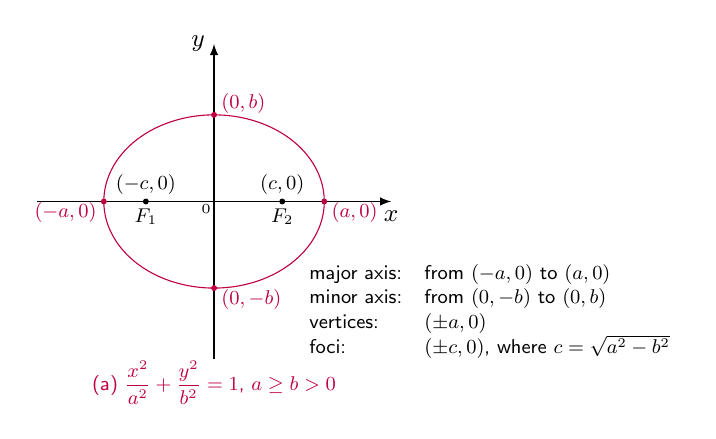
\begin{tikzpicture}[>=latex,xscale=.5*1, yscale=.5*1][font=\sf\small] 

\draw[->] (-4.5, 0) -- (4.5, 0)node[below] {\small $x$};
\draw[->] (0, -4) -- (0, 4)node[left] {\small $y$};

\node[purple, scale=0.8] at (0, -4.6) {(a) $\displaystyle \frac{x^2}{a^2}+\frac{y^2}{b^2}=1$, $a \ge b > 0$};

\node[scale=0.8] at (7, -2.8) {$
\begin{array}{ll}
\hbox{major axis:} &\hbox{from $(-a, 0)$ to $(a, 0)$}\\
\hbox{minor axis:} &\hbox{from $(0, -b)$ to $(0, b)$}\\
\hbox{vertices:} & (\pm a, 0) \\
\hbox{foci:} & \hbox{$(\pm c, 0)$, where $c = \sqrt{a^2-b^2}$} 
\end{array}
$};

\draw[purple, samples=100, smooth, domain=0:2*pi, variable=\t]
		plot ({2.8*cos(\t r)}, {2.2*sin(\t r)}) ;

\draw[fill] ({-sqrt(2.8^2-2.2^2)}, 0) circle(0.06) node[below, scale=0.8]{$F_1$} node[above, scale=0.8]{$(-c, 0)$} ;
\draw[fill] ({ sqrt(2.8^2-2.2^2)}, 0) circle(0.06) node[below, scale=0.8]{$F_2$} node[above, scale=0.8]{$( c, 0)$} ;

\draw[purple, fill] (-2.8,0) circle(0.06) node[left, yshift=-4, scale=0.8]{$(-a,0)$};
\draw[purple, fill] ( 2.8,0) circle(0.06) node[right, yshift=-4, scale=0.8]{$( a,0)$};

\draw[purple, fill] (0, -2.2) circle(0.06) node[right, yshift=-4, scale=0.8]{$(0,-b)$};
\draw[purple, fill] (0,  2.2) circle(0.06) node[right, yshift=4, scale=0.8]{$(0, b)$};

\node at (-0.2/1, -0.2/1) {\tiny$0$};

\end{tikzpicture}
\end{document}